\documentclass[ignorenonframetext,]{beamer}
\usetheme{Madrid}
\usecolortheme{whale}
\setbeamertemplate{caption}[numbered]
\setbeamertemplate{caption label separator}{:}
\setbeamercolor{caption name}{fg=normal text.fg}
\usepackage{amssymb,amsmath}
\usepackage{ifxetex,ifluatex}
\usepackage{fixltx2e} % provides \textsubscript
\usepackage{lmodern}
\ifxetex
  \usepackage{fontspec,xltxtra,xunicode}
  \defaultfontfeatures{Mapping=tex-text,Scale=MatchLowercase}
  \newcommand{\euro}{€}
\else
  \ifluatex
    \usepackage{fontspec}
    \defaultfontfeatures{Mapping=tex-text,Scale=MatchLowercase}
    \newcommand{\euro}{€}
  \else
    \usepackage[T1]{fontenc}
    \usepackage[utf8]{inputenc}
      \fi
\fi
% use upquote if available, for straight quotes in verbatim environments
\IfFileExists{upquote.sty}{\usepackage{upquote}}{}
% use microtype if available
\IfFileExists{microtype.sty}{\usepackage{microtype}}{}
\usepackage{color}
\usepackage{fancyvrb}
\newcommand{\VerbBar}{|}
\newcommand{\VERB}{\Verb[commandchars=\\\{\}]}
\DefineVerbatimEnvironment{Highlighting}{Verbatim}{commandchars=\\\{\}}
% Add ',fontsize=\small' for more characters per line
\usepackage{framed}
\definecolor{shadecolor}{RGB}{248,248,248}
\newenvironment{Shaded}{\begin{snugshade}}{\end{snugshade}}
\newcommand{\KeywordTok}[1]{\textcolor[rgb]{0.13,0.29,0.53}{\textbf{{#1}}}}
\newcommand{\DataTypeTok}[1]{\textcolor[rgb]{0.13,0.29,0.53}{{#1}}}
\newcommand{\DecValTok}[1]{\textcolor[rgb]{0.00,0.00,0.81}{{#1}}}
\newcommand{\BaseNTok}[1]{\textcolor[rgb]{0.00,0.00,0.81}{{#1}}}
\newcommand{\FloatTok}[1]{\textcolor[rgb]{0.00,0.00,0.81}{{#1}}}
\newcommand{\CharTok}[1]{\textcolor[rgb]{0.31,0.60,0.02}{{#1}}}
\newcommand{\StringTok}[1]{\textcolor[rgb]{0.31,0.60,0.02}{{#1}}}
\newcommand{\CommentTok}[1]{\textcolor[rgb]{0.56,0.35,0.01}{\textit{{#1}}}}
\newcommand{\OtherTok}[1]{\textcolor[rgb]{0.56,0.35,0.01}{{#1}}}
\newcommand{\AlertTok}[1]{\textcolor[rgb]{0.94,0.16,0.16}{{#1}}}
\newcommand{\FunctionTok}[1]{\textcolor[rgb]{0.00,0.00,0.00}{{#1}}}
\newcommand{\RegionMarkerTok}[1]{{#1}}
\newcommand{\ErrorTok}[1]{\textbf{{#1}}}
\newcommand{\NormalTok}[1]{{#1}}
\usepackage{longtable,booktabs}
\usepackage{caption}
% These lines are needed to make table captions work with longtable:
\makeatletter
\def\fnum@table{\tablename~\thetable}
\makeatother
\usepackage{graphicx}
\makeatletter
\def\maxwidth{\ifdim\Gin@nat@width>\linewidth\linewidth\else\Gin@nat@width\fi}
\def\maxheight{\ifdim\Gin@nat@height>\textheight0.8\textheight\else\Gin@nat@height\fi}
\makeatother
% Scale images if necessary, so that they will not overflow the page
% margins by default, and it is still possible to overwrite the defaults
% using explicit options in \includegraphics[width, height, ...]{}
\setkeys{Gin}{width=\maxwidth,height=\maxheight,keepaspectratio}

% Comment these out if you don't want a slide with just the
% part/section/subsection/subsubsection title:
\AtBeginPart{
  \let\insertpartnumber\relax
  \let\partname\relax
  \frame{\partpage}
}
\AtBeginSection{
  \let\insertsectionnumber\relax
  \let\sectionname\relax
  \frame{\sectionpage}
}
\AtBeginSubsection{
  \let\insertsubsectionnumber\relax
  \let\subsectionname\relax
  \frame{\subsectionpage}
}

\setlength{\parindent}{0pt}
\setlength{\parskip}{6pt plus 2pt minus 1pt}
\setlength{\emergencystretch}{3em}  % prevent overfull lines
\setcounter{secnumdepth}{0}
\usepackage[russian]{babel}
\author[Эконометрика. Лекция 5]{Эконометрика. Лекция 5}
\newcommand{\e}{\varepsilon}

\title{Гетероскедастичность}
\date{}

\begin{document}
\frame{\titlepage}

\begin{frame}{Гомоскедастичность}

Для проверки гипотез мы предполагали условную гомоскедастичность ошибок:

\(Var(\varepsilon_i | X)=E(\varepsilon_i^2 | X)=\sigma^2\)

Что произойдет если эта предпосылка будет нарушена?

\end{frame}

\begin{frame}{Четыре разных понятия}

Условная гомоскедастичность
\(Var(\varepsilon_i | X)=E(\varepsilon_i^2 | X)=\sigma^2\)

Условная гетероскедастичность
\(Var(\varepsilon_i | X)=E(\varepsilon_i^2 | X) \neq const\)

Безусловная гомоскедастичность
\(Var(\varepsilon_i)=E(\varepsilon_i^2)=\sigma^2\)

Безусловная гетероскедастичность
\(Var(\varepsilon_i)=E(\varepsilon_i^2) \neq \sigma^2\)

\end{frame}

\begin{frame}{Примеры {[}доска{]}}

Имеет ли место условная/безусловная гетероскедастичность в каждом из
случаев?

\begin{itemize}
\itemsep1pt\parskip0pt\parsep0pt
\item
  Случай А: \(\e_i\) независимы и одинаково распределены
\end{itemize}

\begin{longtable}[c]{@{}lllll@{}}
\toprule
Вероятности & \(\e_i=-10\) & \(\e_i=-1\) & \(\e_i=1\) &
\(\e_i=10\)\tabularnewline
\midrule
\endhead
\(x_i=1\) & 0 & 1/4 & 1/4 & 0\tabularnewline
\(x_i=10\) & 0 & 1/4 & 1/4 & 0\tabularnewline
\bottomrule
\end{longtable}

\begin{itemize}
\itemsep1pt\parskip0pt\parsep0pt
\item
  Случай B: \(\e_i\) независимы и одинаково распределены
\end{itemize}

\begin{longtable}[c]{@{}lllll@{}}
\toprule
Вероятности & \(\e_i=-10\) & \(\e_i=-1\) & \(\e_i=1\) &
\(\e_i=10\)\tabularnewline
\midrule
\endhead
\(x_i=1\) & 0 & 1/4 & 1/4 & 0\tabularnewline
\(x_i=10\) & 1/4 & 0 & 0 & 1/4\tabularnewline
\bottomrule
\end{longtable}

\end{frame}

\begin{frame}{Примеры {[}доска{]}}

Имеет ли место условная/безусловная гетероскедастичность в каждом из
случаев?

\begin{itemize}
\itemsep1pt\parskip0pt\parsep0pt
\item
  Случай C: \(\e_i\) независимы
\end{itemize}

\begin{longtable}[c]{@{}lllll@{}}
\toprule
Вероятности & \(\e_1=-10\) & \(\e_1=-1\) & \(\e_1=1\) &
\(\e_1=10\)\tabularnewline
\midrule
\endhead
\(x_1=1\) & 0 & 1/4 & 1/4 & 0\tabularnewline
\(x_1=10\) & 0 & 1/4 & 1/4 & 0\tabularnewline
\bottomrule
\end{longtable}

\begin{longtable}[c]{@{}lllll@{}}
\toprule
Вероятности & \(\e_2=-10\) & \(\e_2=-1\) & \(\e_2=1\) &
\(\e_2=10\)\tabularnewline
\midrule
\endhead
\(x_2=1\) & 1/4 & 0 & 0 & 1/4\tabularnewline
\(x_2=10\) & 1/4 & 0 & 0 & 1/4\tabularnewline
\bottomrule
\end{longtable}

\end{frame}

\begin{frame}{Когда логично ожидать гетероскедастичность?}

\begin{itemize}
\item
  безусловной в случайной выборке не бывает
\item
  условная возникает при наличии ``размера'' объекта
\item
  условная присутствует почти всегда
\end{itemize}

\end{frame}

\begin{frame}{В остальном всё ок}

Предпосылка об условной гомоскедастичности нарушена.

Все остальные предпосылки классической модели со стохастическими
регрессорами для случайной выборки выполнены.

\end{frame}

\begin{frame}{Мы используем прежние формулы:}

Для оценок коэффициентов:

\(\hat{\beta}=(X'X)^{-1}X'y\)

Для оценки ковариационной матрицы оценок коэффициентов:

\(\widehat{Var}(\hat{\beta}|X)=\frac{RSS}{n-k}(X'X)^{-1}\)

В частности:

\(\widehat{Var}(\hat{\beta}_j|X)=\frac{\hat{\sigma}^2}{RSS_j}\) и
\(se(\hat{\beta}_j)=\sqrt{\widehat{Var}(\hat{\beta}_j|X)}\)

\end{frame}

\begin{frame}{Три группы свойств:}

\begin{itemize}
\item
  конечная выборка без предположения о нормальности \(\varepsilon\)
\item
  конечная выборка с предположением о нормальности \(\varepsilon\)
\item
  асимптотические свойства без предположения о нормальности
  \(\varepsilon\)
\end{itemize}

Что происходит в каждом случае?

\end{frame}

\begin{frame}{Малая выборка без нормальности \(\varepsilon\)}

\begin{itemize}
\item
  (+) Линейность по \(y\)
\item
  (+) Несмещенность, \(E(\hat{\beta}|X)=\beta\),
  \(E(\hat{\beta})=\beta\)
\item
  (---) Оценки \(\hat{\beta}\) эффективны
\end{itemize}

\end{frame}

\begin{frame}{Малая выборка с нормальными \(\varepsilon\)}

\begin{itemize}
\item
  (---)
  \(\frac{\hat{\beta}_j-\beta_j}{se(\hat{\beta}_j)} | X \sim t_{n-k}\)
\item
  (---) \(\frac{RSS}{\sigma^2} |X \sim \chi^2_{n-k}\)
\item
  (---) \(\frac{(RSS_R-RSS_{UR})/r}{RSS_{UR}/(n-k)} \sim F_{r,n-k}\)
\end{itemize}

\end{frame}

\begin{frame}{Асимптотические свойства}

\begin{itemize}
\item
  (+) \(\hat{\beta} \to \beta\)
\item
  (+) \(\frac{RSS}{n-k} \to \sigma^2=Var(\e_i)\)
\item
  (---) \(\frac{\hat{\beta}_j-\beta_j}{se(\hat{\beta}_j)} \to N(0,1)\)
\item
  (---) \(\frac{RSS_R-RSS_{UR}}{RSS_{UR}/(n-k)} \to \chi^2_r\)
\end{itemize}

\end{frame}

\begin{frame}{Мораль:}

\begin{itemize}
\item
  Сами \(\hat{\beta}\) можно интерпретировать и использовать
\item
  Стандартные ошибки \(se(\hat{\beta}_j)\) несостоятельны
\item
  Не можем строить доверительные интервалы для \(\beta_j\) и проверять
  гипотезы
\end{itemize}

\end{frame}

\begin{frame}{Что делать?}

\begin{itemize}
\item
  Исправить стандартные ошибки!
\item
  Другая формула для оценки \(\widehat{Var}_{HC}(\hat{\beta}|X)\)
\item
  Следовательно, другие \(se_{HC}(\hat{\beta}_j)\)
\end{itemize}

\end{frame}

\begin{frame}{Робастная (устойчивая) к гетероскедастичности оценка
ковариационной матрицы}

\begin{itemize}
\itemsep1pt\parskip0pt\parsep0pt
\item
  Вместо
\end{itemize}

\(\widehat{Var}(\hat{\beta}|X)=\frac{RSS}{n-k}(X'X)^{-1}\)

использовать

\(\widehat{Var}_{HC}(\hat{\beta}|X)=(X'X)^{-1}X'\hat{\Omega}X(X'X)^{-1}\)

\begin{itemize}
\itemsep1pt\parskip0pt\parsep0pt
\item
  Уайт, 1980, HC0:
\end{itemize}

\(\hat{\Omega}=diag( \hat{\varepsilon}_1^2, \ldots, \hat{\varepsilon}_n^2 )\)

\begin{itemize}
\itemsep1pt\parskip0pt\parsep0pt
\item
  Современный вариант, HC3:
\end{itemize}

\(\hat{\Omega}=diag \left( \frac{\hat{\varepsilon}_1^2}{(1-h_{11})^2}, \ldots, \frac{\hat{\varepsilon}_n^2}{(1-h_{nn})^2} \right)\)

\end{frame}

\begin{frame}{Суть корректировки:}

Мы меняем \(se(\hat{\beta}_j)\) на \(se_{HC}(\hat{\beta}_j)\)

Какие проблемы решены?

\begin{itemize}
\itemsep1pt\parskip0pt\parsep0pt
\item
  (+)
  \(\frac{\hat{\beta}_j-\beta_j}{se_{HC}(\hat{\beta}_j)} \to N(0,1)\)
  (УРА!)
\end{itemize}

\end{frame}

\begin{frame}{Какие проблемы не решены?}

\begin{itemize}
\itemsep1pt\parskip0pt\parsep0pt
\item
  (---) эффективность
\end{itemize}

Оценки \(\hat{\beta}\) не меняются и остаются неэффективными!

Даже при предположении о нормальности \(\varepsilon\):

\begin{itemize}
\item
  (---)
  \(\frac{\hat{\beta}_j-\beta_j}{se_{HC}(\hat{\beta}_j)} | X \sim t_{n-k}\)
\item
  (---) \(\frac{RSS}{\sigma^2} |X \sim \chi^2_{n-k}\)
\item
  (---) \(\frac{(RSS_R-RSS_{UR})/r}{RSS_{UR}/(n-k)} \sim F_{r,n-k}\)
\end{itemize}

\end{frame}

\begin{frame}[fragile]{С практической точки зрения:}

\begin{itemize}
\item
  Новая формула для \(\widehat{Var}_{HC}(\hat{\beta}|X)\), и,
  следовательно, для \(se_{HC}(\hat{\beta}_j)\)
\item
  робастная ковариационная матрица в R (по умолчанию HC3):
\end{itemize}

\begin{Shaded}
\begin{Highlighting}[]
\NormalTok{model <-}\StringTok{ }\KeywordTok{lm}\NormalTok{(y~x, }\DataTypeTok{data=}\NormalTok{data)}
\KeywordTok{vcovHC}\NormalTok{(model)}
\end{Highlighting}
\end{Shaded}

\begin{itemize}
\itemsep1pt\parskip0pt\parsep0pt
\item
  С ней жизнь прекрасна!
\end{itemize}

(+) \(\frac{\hat{\beta}_j-\beta_j}{se_{HC}(\hat{\beta}_j)} \to N(0,1)\)

\end{frame}

\begin{frame}{Когда следует использовать робастные стандартные ошибки?}

\begin{itemize}
\itemsep1pt\parskip0pt\parsep0pt
\item
  Как только есть случайная выборка и объекты могут быть разного
  ``размера'', использовать \(se_{HC}(\hat{\beta}_j)\) для проверки
  гипотез!
\end{itemize}

\end{frame}

\begin{frame}{Обнаружение гетероскедастичности}

\begin{itemize}
\item
  Оцениваем интересующую нас модель с помощью МНК
\item
  Строим график квадратов (или модулей) остатков в зависимости от
  регрессора
\end{itemize}

\end{frame}

\begin{frame}{Условная гомоскедастичность}

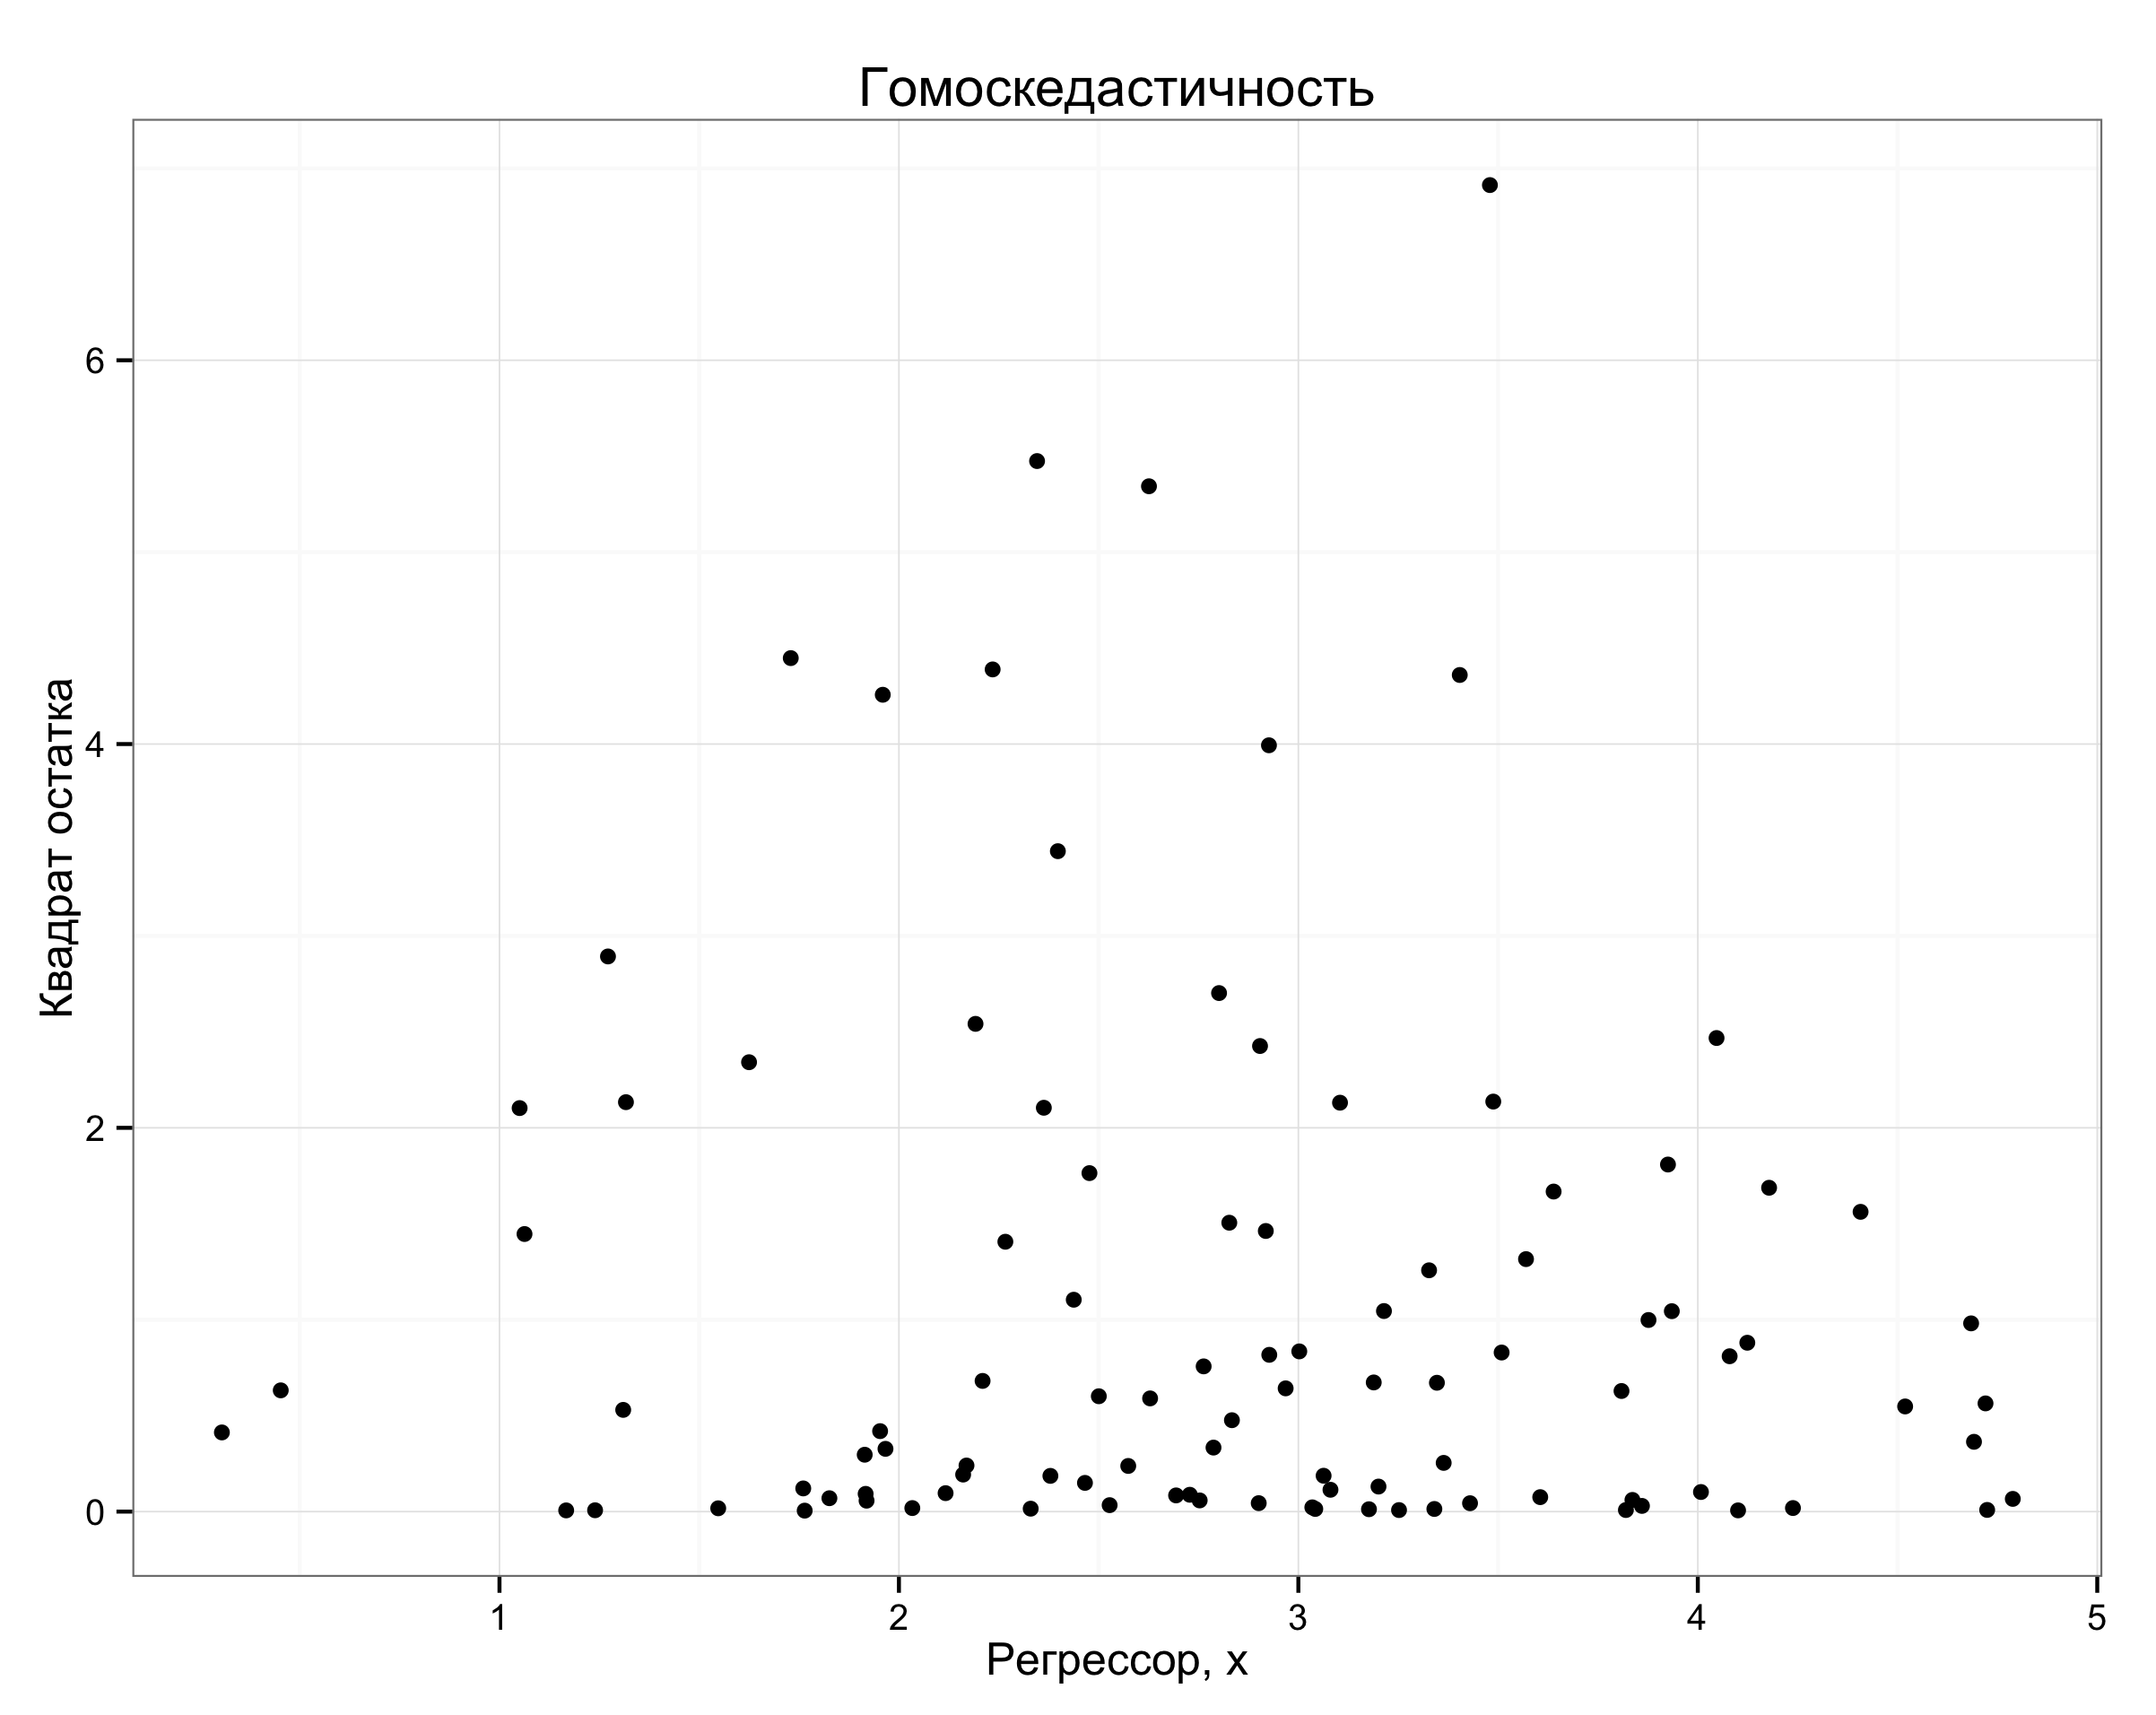
\includegraphics{graph_01_gomo.png}

\end{frame}

\begin{frame}{Условная гетероскедастичность}

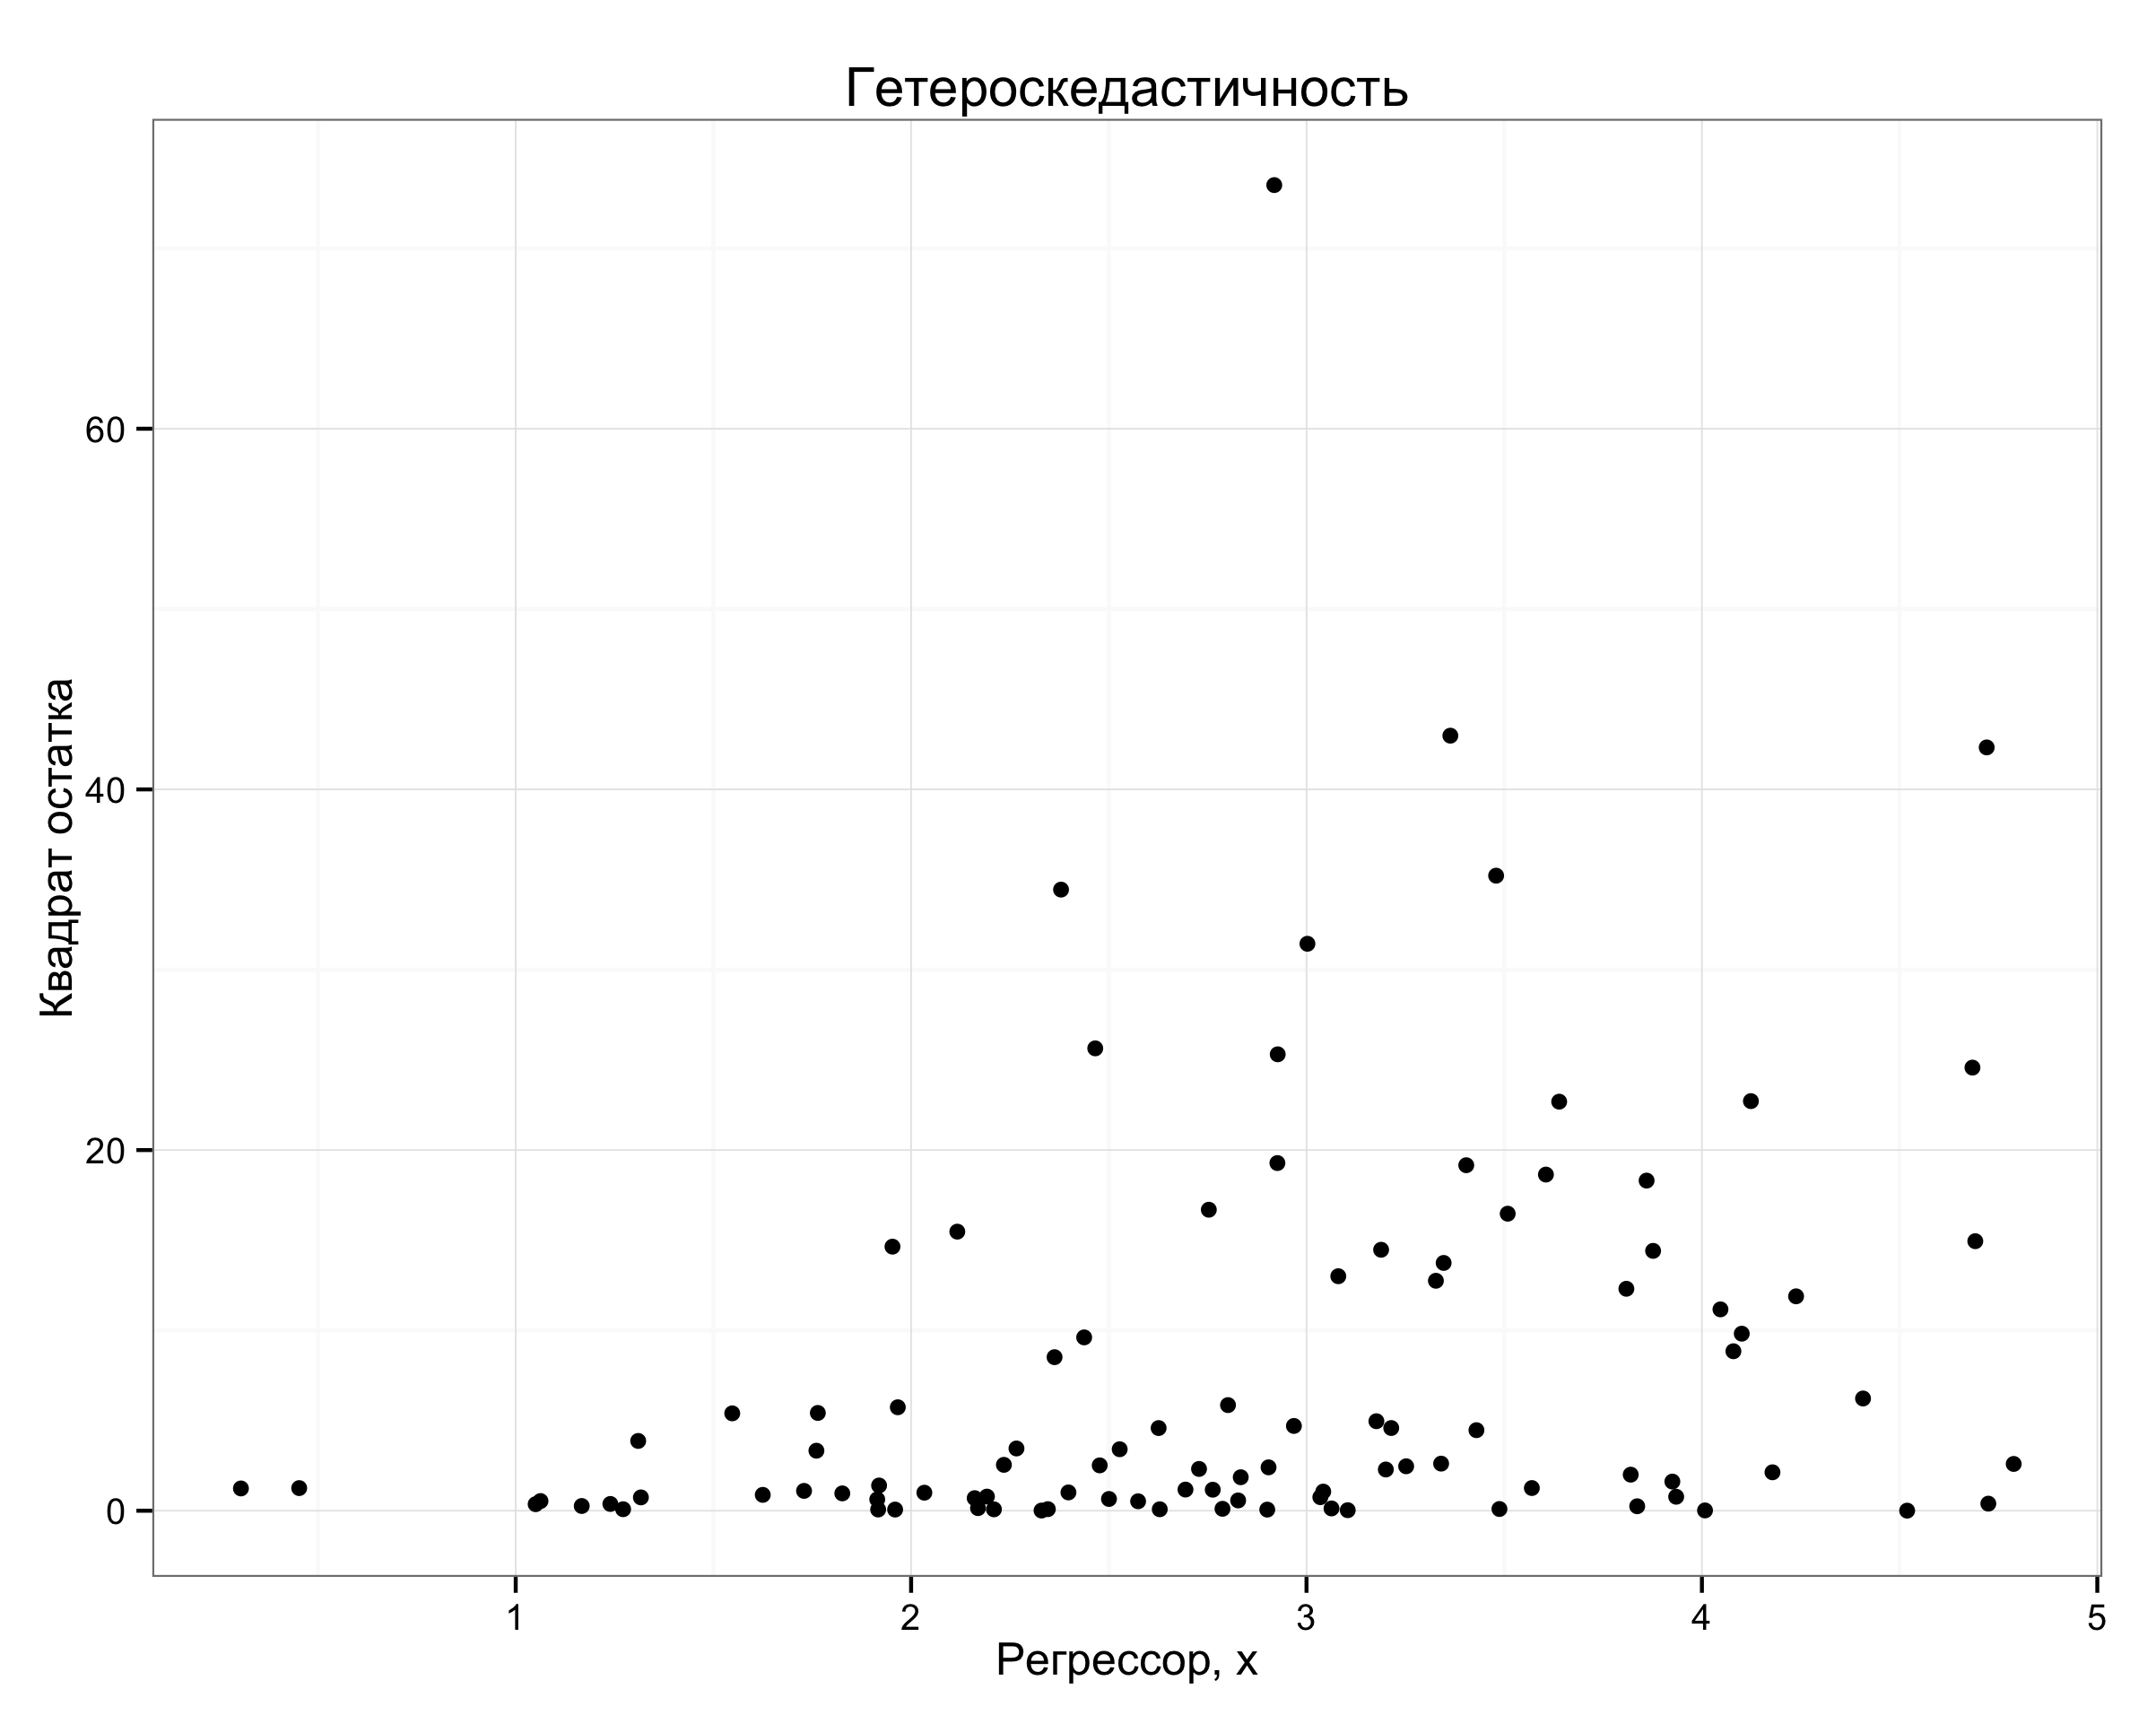
\includegraphics{graph_02_getero.png}

\end{frame}

\begin{frame}{Формальные тесты на гетероскедастичность}

\begin{itemize}
\item
  Тест Уайта (White)
\item
  Тест Голдфельда-Квандта (Goldfeld-Quandt)
\end{itemize}

\end{frame}

\begin{frame}{Тест Уайта}

\begin{itemize}
\item
  асимптотический
\item
  не требуется нормальность остатков
\end{itemize}

\end{frame}

\begin{frame}{Тест Уайта, алгоритм}

\begin{enumerate}
\def\labelenumi{\arabic{enumi}.}
\item
  Оценить основную регрессию, получить \(\hat{\varepsilon}_i\)
\item
  Оценить вспомогательную регрессию:
\end{enumerate}

\(\hat{\varepsilon}^2_i = \gamma_1 + \gamma_2 z_{i2} + \ldots + \gamma_{m} z_{im}+ u_i\)

\(z_{i2}\), \ldots, \(z_{im}\) --- факторы, определяющие форму
гетероскедастичности.

По умолчанию во вспомогательной регрессии берут исходные регрессоры, их
квадраты и попарные произведения

\begin{enumerate}
\def\labelenumi{\arabic{enumi}.}
\setcounter{enumi}{2}
\itemsep1pt\parskip0pt\parsep0pt
\item
  Посчитать \(LM=nR^2_{aux}\)
\end{enumerate}

\end{frame}

\begin{frame}{Тест Уайта}

При верной \(H_0\) об условной гомоскедастичности:

\(H_0\): \(Var(\e_i|X)=E(\varepsilon^2_i|X)=\sigma^2\)

\(LM \sim \chi^2_{m-1}\), где \(m\) --- число параметров во
вспомогательной регрессии

Если наблюдаемое значение статистики \(LM\) больше критического
\(\chi^2_{cr}\), то \(H_0\) отвергается.

\end{frame}

\begin{frame}{Тест Уайта {[}доска{]}}

По 200 киоскам мороженого и исследователь оценил зависимость спроса (q)
от цены (p), разнообразия ассортимента (a) и удаленности от метро (d).

\begin{itemize}
\itemsep1pt\parskip0pt\parsep0pt
\item
  Какой регрессор скорее всего влияет на условную дисперсию ошибок?
\end{itemize}

Исследователь провел классический тест Уайта и получил
\(R^2_{aux}=0.2\).

\begin{itemize}
\item
  Как выглядит вспомогательная регрессия для теста Уайта?
\item
  Имеет ли место условная гетероскедастичность?
\end{itemize}

\end{frame}

\begin{frame}{Тест Голдфельда-Квандта (Goldfeld-Quandt)}

\begin{itemize}
\item
  Есть переменная, от которой условная дисперсия ошибок предположительно
  зависит монотонно
\item
  Требуется нормальность ошибок
\item
  Тест подходит для малых выборок
\end{itemize}

\end{frame}

\begin{frame}{Процедура теста Голдфельда-Квандта}

\begin{enumerate}
\def\labelenumi{\arabic{enumi}.}
\item
  Сортируем наблюдения по предполагаемому убыванию условной дисперсии
\item
  Выкидываем часть наблюдений посередине (например, 20\%)
\item
  Оцениваем исходную модель отдельно по первым и по последним
  наблюдениям
\item
  Считаем \(F=\frac{RSS_1/(n_1-k)}{RSS_2/(n_2-k)}\)
\end{enumerate}

\end{frame}

\begin{frame}{Тест Голдфельда-Квандта продолжение}

При верной \(H_0\) об условной гомоскедастичности:

\(H_0\): \(Var(\e_i|X)=E(\varepsilon^2_i|X)=\sigma^2\)

\(F\sim F_{n_1-k,n_2-k}\)

Если наблюдаемое значение статистики \(F\) больше критического
\(F_{cr}\), то \(H_0\) отвергается.

\end{frame}

\begin{frame}{Тест Голдфельда-Квандта {[}доска{]}}

По 200 киоскам мороженого и исследователь оценил зависимость спроса (q)
от цены (p), разнообразия ассортимента (a) и удаленности от метро (d).

Чтобы проверить наличие гетероскедастичности исследователь оценил эту
модель отдельно по 80 самым удаленным от метро киоскам, получил,
\(RSS_2=120\). По 80 самым близки к метро киоскам, получил,
\(RSS_1=210\).

Проведите тест Голдфельда-Квандта

\end{frame}

\begin{frame}{Эффективность оценок?}

\begin{itemize}
\item
  Да, надо смириться с тем, что оценки неэффективны
\item
  Мы довольны несмещенностью, состоятельностью и возможностью проверять
  гипотезы
\item
  Для получения эффективных оценок нужно точно понимать как устроена
  гетероскедастичность. Это большая редкость.
\end{itemize}

\end{frame}

\begin{frame}{Получение эффективных оценок {[}доска{]}}

Модель \(m_i = \beta_1 + \beta_2 r_i + \beta_3 t_i + \e_i\):

\begin{itemize}
\item
  \(m_i\) --- средний результат класса по математике
\item
  \(r_i\) --- количество учеников
\item
  \(t_i\) --- среднее время, потраченное на занятия математикой
\item
  Какую структуру гетероскедастичности логично ожидать?
\item
  Как при такой структуре гетероскедастичности получить эффективные
  оценки?
\end{itemize}

\end{frame}

\begin{frame}{Мораль}

\begin{itemize}
\item
  Нарушение предпосылки об условной гомоскедастичности
\item
  Почти всегда имеет место в случайной выборке
\item
  Неприятность небольшая, мы используем робастные стандартные ошибки
\item
  Если нужны эффективные оценки, то надо знать структуру
  гетероскедастичности
\end{itemize}

\end{frame}

\end{document}
